\subsection*{Цель работы}
Исследовать характеристики фоторезистора при внутреннем фотоэффекте; найти ширину запрещенной зоны полупроводника.

\subsection*{Приборы и принадлежности}
Модульный учебный комплекс МУК-ОК, в состав которого входят стенд с объектами исследования С3-ОК01, амперметр-вольтметр АВ-1, источник питания ИПС1, набор светодиодов (кластер), соединительные проводники.

% \begin{figure}[H]
%     \def\thefigure{7.6}
%     \protect\phantomsection
    
%     \centering
%     \includegraphics[width=0.5\linewidth]{figs/2.png}
%     \caption{Модульный учебный комплекс МУК-ОК}
%     \label{fig:placeholder}
% \end{figure}

\subsection*{Исследуемые закономерности}
Принцип действия фоторезистора основан на явлении внутреннего фотоэффекта --- увеличении электропроводности полупроводника под действием света. Световые кванты (фотоны) с достаточной энергией создают в полупроводнике дополнительные пары носителей заряда (электрон-дырка), что приводит к уменьшению его сопротивления.

% \begin{figure}[H]
%     \def\thefigure{7.5}
%     \protect\phantomsection 
    
%     \centering
%     \includegraphics[width=0.5\linewidth]{figs/12.png}
%     \caption{Электрическая схема экспериментальной установки}
%     \label{fig:элсхема}
% \end{figure}

\subsubsection*{Основные характеристики и формулы для расчетов:}
\begin{enumerate}
    \item \textbf{Фототок ($I_\text{ф}$):} Измеряемый в цепи ток $I$ является суммой темнового тока $I_\text{т}$ (существующего без освещения) и фототока $I_\text{ф}$ (возникающего под действием света). Для анализа используется именно фототок:
    \[ I_\text{ф} = I - I_\text{т} \]
    
    \item \textbf{Вольт-амперная характеристика (ВАХ):} Зависимость фототока от приложенного напряжения при постоянной освещенности и длине волны света.
    \[ I_\text{ф} = f(U) \quad \text{при} \quad \Phi, \lambda = \text{const} \]
    Для фоторезистора эта зависимость является линейной.
    
    \item \textbf{Световая характеристика:} Зависимость фототока от интенсивности падающего светового потока $\Phi$ при постоянном напряжении.
    \[ I_\text{ф} = f(\Phi) \quad \text{при} \quad U, \lambda = \text{const} \]
    Характеристика является нелинейной, с тенденцией к насыщению при больших интенсивностях.
    
    \item \textbf{Спектральная характеристика:} Зависимость фототока от длины волны $\lambda$ падающего света.
    \[ I_\text{ф} = f(\lambda) \quad \text{при} \quad U, \Phi = \text{const} \]
    Эта зависимость имеет максимум и резкий спад в длинноволновой области. Точка спада позволяет определить \textbf{красную границу} фотоэффекта $\lambda_\text{гр}$.
    
    \item \textbf{Ширина запрещенной зоны ($\Delta\varepsilon$):} Энергия фотона, соответствующая красной границе, равна ширине запрещенной зоны полупроводника. Она вычисляется по формуле:
    \[ \Delta\varepsilon = \frac{hc}{\lambda_\text{гр}} \]
    где $h = 6.626 \cdot 10^{-34}$~Дж$\cdot$с --- постоянная Планка, $c = 3 \cdot 10^8$~м/с --- скорость света в вакууме. Для перевода в электрон-вольты (эВ) результат нужно разделить на заряд электрона $e = 1.6 \cdot 10^{-19}$~Кл.
\end{enumerate}










\newpage
\centeredsection{\MakeUppercase{Указания по проведению эксперимента}}
\begin{enumerate}
    \item С помощью коммутации проводников собрать электрическую схему согласно рис.~7.5.
    
    \item Включить приборы. Установить начальные параметры интенсивности и выбрать режимы измерения на вольтметре и амперметре.
    
    \item \textbf{Снять темновую характеристику:} Измерить зависимость темнового тока $I_\text{т}$ от напряжения $U$ при выключенных светодиодах (или минимальной интенсивности $\Phi \approx 0$).
    
    \item \textbf{Снять вольт-амперные характеристики:} Для трех различных длин волн ($\lambda_1, \lambda_2, \lambda_3$) при фиксированном световом потоке $\Phi$ измерить зависимость общего тока $I$ от напряжения $U$.
    
    \item \textbf{Снять световые характеристики:} Для двух длин волн ($\lambda_1, \lambda_2$) при фиксированном напряжении $U$ измерить зависимость общего тока $I$ от относительной интенсивности светового потока $\Phi = J/J_0$.
    
    \item \textbf{Снять спектральную характеристику:} При фиксированных напряжении $U$ и световом потоке $\Phi$ измерить общий ток $I$ для всех доступных длин волн $\lambda$ (светодиодов).
\end{enumerate}







































\newpage
\thispagestyle{empty}
\centeredsection{ПРОТОКОЛ НАБЛЮДЕНИЙ}

% \begin{table}[H]
%     \centering
%     \caption{Вольт-амперные характеристики \\($\Phi = J/J_0 = $ \underline{\hspace{1.5cm}}, $\lambda_1 = $ \underline{\hspace{1cm}} нм, $\lambda_2 = $ \underline{\hspace{1cm}} нм, $\lambda_3 = $ \underline{\hspace{1cm}} нм)}
%     \tiny % Уменьшаем шрифт, чтобы таблица поместилась
%     \begin{tabularx}{\linewidth}{|L|C|C|C|C|C|C|C|C|C|C|C|C|}
%         \hline
%             $U$, В & 0.5 & 1.0 & 1.5 & 2.0 & 2.5 & 3.0 & 3.5 & 4.0 & 4.5 & 5.0 & 5.5 & 6.0 \\
%         \hline
%             $I_\text{т}$, мкА & & & & & & & & & & & & \\
%         \hline \hline
%             $I (\lambda_1)$, мкА & & & & & & & & & & & & \\
%         \hline
%             $I_\text{ф}(\lambda_1)$, мкА & & & & & & & & & & & & \\
%         \hline \hline
%             $I (\lambda_2)$, мкА & & & & & & & & & & & & \\
%         \hline
%             $I_\text{ф}(\lambda_2)$, мкА & & & & & & & & & & & & \\
%         \hline \hline
%             $I (\lambda_3)$, мкА & & & & & & & & & & & & \\
%         \hline
%             $I_\text{ф}(\lambda_3)$, мкА & & & & & & & & & & & & \\
%         \hline
%     \end{tabularx}
% \end{table}
\begin{table}[H]
    \centering
    \caption{Вольт-амперные характеристики \\($\Phi = J/J_0 = $ \underline{\hspace{1.5cm}}, $\lambda_1 = $ \underline{\hspace{1cm}} нм, $\lambda_2 = $ \underline{\hspace{1cm}} нм, $\lambda_3 = $ \underline{\hspace{1cm}} нм)}
    \begin{tabularx}{\linewidth}{|C|C|C|C|C||C|C|C|C|C|}
        \hline
        $U$, В & $I_\text{т}$ & $I(\lambda_1)$ & $I(\lambda_2)$ & $I(\lambda_3)$ & $U$, В & $I_\text{т}$ & $I(\lambda_1)$ & $I(\lambda_2)$ & \textbf{$I(\lambda_3)$} \\
        \hline
        0.5 & & & & & 3.5 & & & & \\
        \hline
        1.0 & & & & & 4.0 & & & & \\
        \hline
        1.5 & & & & & 4.5 & & & & \\
        \hline
        2.0 & & & & & 5.0 & & & & \\
        \hline
        2.5 & & & & & 5.5 & & & & \\
        \hline
        3.0 & & & & & 6.0 & & & & \\
        \hline
    \end{tabularx}
\end{table}


\begin{table}[H]
    \centering
    \caption{Световые характеристики \\($U = $ \underline{\hspace{1.5cm}} В, $I_\text{т} = $ \underline{\hspace{1.5cm}} мкА, $\lambda_1 = $ \underline{\hspace{1cm}} нм, $\lambda_2 = $ \underline{\hspace{1cm}} нм)}
    \begin{tabularx}{\linewidth}{|C|C|C||C|C|C|}
        \hline
        $\Phi = J/J_0$ & $I(\lambda_1)$ & $I(\lambda_2)$ & $\Phi = J/J_0$ & $I(\lambda_1)$ & $I(\lambda_2)$ \\
        \hline
        0.1 & & & 0.7 & & \\
        \hline
        0.2 & & & 0.8 & & \\
        \hline
        0.3 & & & 0.9 & & \\
        \hline
        0.4 & & & 1.0 & & \\
        \hline
        0.5 & & & 1.1 & & \\
        \hline
        0.6 & & & 1.2 & & \\
        \hline
    \end{tabularx}
\end{table}



\begin{table}[H]
    \centering
    \caption{Спектральная характеристика \\($U = $ \underline{\hspace{1.5cm}} В, $\Phi = J/J_0 = $ \underline{\hspace{1.5cm}}, $I_\text{т} = $ \underline{\hspace{1.5cm}} мкА)}
    
    \begin{tabularx}{\linewidth}{|L|C|C|C|C|C|C|C|C|}
        \hline
        $\lambda$, нм & 430 & 470 & 520 & 565 & 590 & 660 & 700 & 860 \\
        \hline
        $I$, мкА & & & & & & & & \\
        \hline
        $I_\text{ф}$, мкА & & & & & & & & \\
        \hline
    \end{tabularx}
\end{table}


\vfill
\noindent
Рахметов А. Р., гр. 4494 ~~\hrulefill~~ «\rule{1cm}{0.4pt}» \rule{3cm}{0.4pt} 20\rule{0.75cm}{0.4pt} г.

% \newpage
% \centeredsection{Вопросы}
% \section*{Вопрос 1 (№19).}
% \begin{quote}
%     \textit{Сформулируйте принцип суперпозиции волн.}
% \end{quote}

% Принцип суперпозиции утверждает, что если в среде одновременно распространяется несколько волн, то результирующее смещение среды в любой точке и в любой момент времени равно векторной сумме смещений, которые создавала бы каждая из волн в отдельности.

% \begin{equation*}
%     \vec{E} = \sum_{i=1}^{n} \vec{E}_i
% \end{equation*}



% \section*{Вопрос 2 (№37).}
% \begin{quote}
%     \textit{Какова интерференция при отражении света от плоскопараллельной пластинки? Покажите ход лучей. Рассчитайте оптическую разность хода.}
% \end{quote}
% \begin{figure}[H]
%     \centering
%     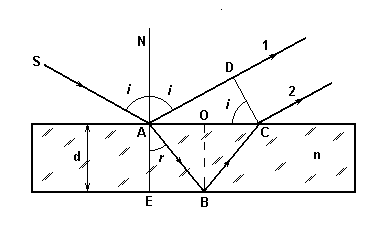
\includegraphics[width=0.5\linewidth]{interferenc.png}
% \end{figure}
% Лучи (1) и (2) являются когерентными (т.е. колебания происходят синхронно; т.к. они произошли от одного исходного луча) и распространяются параллельно друг другу. Их интерференция наблюдается в плоскости, перпендикулярной лучам (1) и (2).

% Оптическая разность хода (разность хода; $\Delta$) --- это разница между оптическими длинами путей, пройденных двумя когерентными световыми волнами от общего источника до одной и той же точки: $\Delta = l_2-l_1=l_1-l_2$; $\Delta = m\lambda$ (для max); $\Delta = (m+\frac12)\lambda$ (для min), где $l_\text{опт}=n\cdot l_\text{геом}$.

% Оптическая длина пути --- расстояние, на которое свет распространился бы в вакууме за время его прохождения между данными двумя точками.

% Для примера выше оптическая разность хода будет равна: $\Delta=2nd\cos(i')+\frac{\lambda}2$.

% \newpage
% \centeredsection{ИДЗ №33}
% \begin{quote}
%     Пучок монохроматических ($\lambda= 600$ нм) световых волн падает под углом $\alpha= 30^\circ$ на находящуюся в воздухе мыльную плёнку ($n = 1,30$). При какой наименьшей толщине $d$ плёнки отражённые световые волны будут: 1) максимально ослаблены интерференцией; 2) максимально  усилены?
% \end{quote}
% \begin{figure}[H]
%     \centering
%     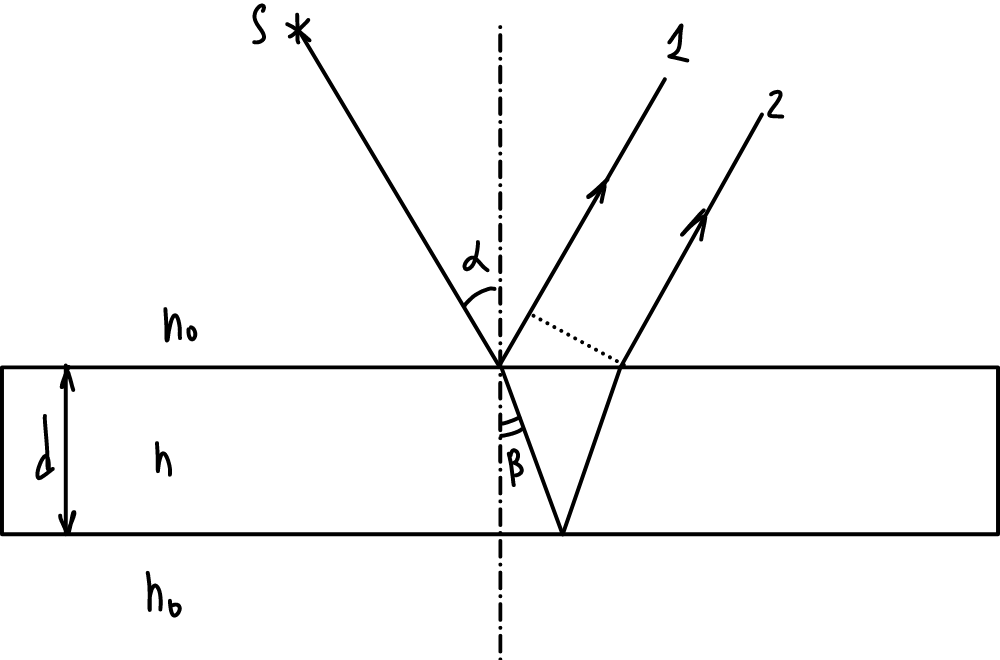
\includegraphics[width=0.5\linewidth]{IMG_20250928_220659_551.jpg}
% \end{figure}

% \begin{enumerate}
%     \item Рассчитаем $\cos\beta$
%         $$n_0\sin\alpha=n\sin\beta\Rightarrow\sin\beta=\frac{n_0\sin\alpha}{n}=\frac{1\cdot\sin(30^\circ)}{1,3}=\frac{5}{13}$$

%         $$\cos\beta=\sqrt{1-\sin^2\beta}=\sqrt{\frac{144}{169}}=\frac{12}{13}$$

%         $$\cos\beta=\frac{12}{13}$$

%     \item Найдем разность хода
%         $$l_1=\frac\lambda2;\qquad l_2=2nd\cos\beta;\qquad \Delta=l_2-l_1$$
%         $$\Delta=2nd\cos\beta-\frac{\lambda}{2}$$
%     \item Максимальное ослабление ($\Delta=(m+\frac12)\lambda$)
%         $$2nd\cos\beta-\frac{\lambda}{2} = (m+\frac12)\lambda$$
%         $$2nd\cos\beta = (m+\frac12)\lambda + \frac{\lambda}{2}$$
%         $$2nd\cos\beta = (m+1)\lambda, m\in\mathbb{Z} \Rightarrow m+1\equiv m$$
%         $$2nd\cos\beta = m\lambda$$
%         $$d = \frac{m\lambda}{2n\cos\beta},~~d_{min}\text{ при } m=1$$
%         $$d = \frac{\lambda}{2n\cos\beta}$$
%         $$d_{min} = \frac{600\text{ нм}}{2\cdot 1,3 \cdot \frac{12}{13}}=250\text{ нм}$$
%         $$\boxed{d_{min, \text{ослабление}} = 250\text{ нм}}$$
%     \item Максимальное усиление ($\Delta=m\lambda$)
%         $$2nd\cos\beta-\frac{\lambda}{2} = m\lambda$$
%         $$2nd\cos\beta = m\lambda + \frac{\lambda}{2}$$
%         $$2nd\cos\beta = (m+\frac12)\lambda$$
%         $$d = \frac{(m+\frac12)\lambda}{2n\cos\beta},~~d_{min}\text{ при } m=0$$
%         $$d_{min} = \frac{\frac12\lambda}{2n\cos\beta}$$
%         $$d_{min} = \frac{\frac{1}{2}\cdot600\text{ нм}}{2\cdot 1,3 \cdot \frac{12}{13}}=125\text{ нм}$$
%         $$\boxed{d_{min, \text{усиление}} = 125\text{ нм}}$$
        
% \end{enumerate}